\documentclass{standalone}
\usepackage{amssymb,amsmath,latexsym, braket}
\usepackage{tikz, pgfplots, graphicx}
\begin{document}
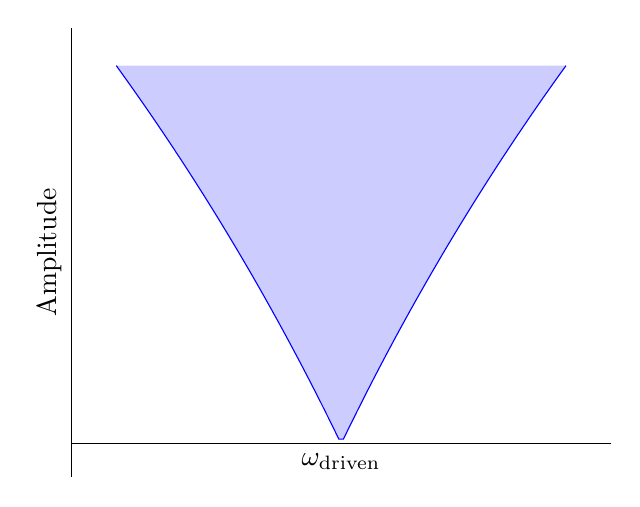
\begin{tikzpicture}
    \begin{axis}[domain=0:4,range=0:1,legend pos=south east,
    axis lines*=middle,
    xlabel=$\omega_{\rm driven}$,
    ylabel=Amplitude,
    xtick={2},
    xticklabels={$\omega_{\rm driving}$},
    ytick={0},
    yticklabels={$0$}
    axis lines = middle,
%every axis x label/.style={at={(current axis.right of origin)},anchor=west},
%every axis y label/.style={at={(current axis.north west)},above=2mm},
     ]
	    \addplot[samples=100, mark=none,domain=0.5:1.5, color=blue,fill=blue!20] {(x<1)*ln(2-x) + (x>1)*ln(x)};
    \end{axis}
\end{tikzpicture}
\end{document}